\documentclass{beamer}
\usepackage[utf8]{inputenc}

\usetheme{Madrid}
\usecolortheme{default}
\usepackage{amsmath,amssymb,amsfonts,amsthm}
\usepackage{txfonts}
\usepackage{tkz-euclide}
\usepackage{listings}
\usepackage{adjustbox}
\usepackage{array}
\usepackage{tabularx}
\usepackage{gvv}
\usepackage{lmodern}
\usepackage{circuitikz}
\usepackage{tikz}
\usepackage{graphicx}

\setbeamertemplate{page number in head/foot}[totalframenumber]

\usepackage{tcolorbox}
\tcbuselibrary{minted,breakable,xparse,skins}

% Code styling
\lstset{
    language=C,
    basicstyle=\ttfamily\small,
    keywordstyle=\color{blue},
    stringstyle=\color{orange},
    commentstyle=\color{green!60!black},
    numbers=left,
    numberstyle=\tiny\color{gray},
    breaklines=true,
    showstringspaces=false,
}
%------------------------------------------------------------

\title
{1.6.23}
\date{September 14, 2025}
\author 
{AI25BTECH11008\\Chiruvella Harshith Sharan}

\begin{document}

\frame{\titlepage}

\begin{frame}{Question}
\centering
Are the points A(3,1), B(6,4), and C(8,6) collinear?
\end{frame}

\begin{frame}{Theoretical Solution}
$\vec{B}-\vec{A}=\myvec{6-3 \\ 4-1} = \myvec{3 \\ 3}$ \\
$\vec{C}-\vec{A}=\myvec{8-3 \\ 6-1} = \myvec{5 \\ 5}$ \\\\

Clearly, $\vec{C}-\vec{A} = \tfrac{5}{3}(\vec{B}-\vec{A})$ \\
$\implies$ The two vectors are linearly dependent. \\\\

\begin{align}
\centering
\boxed{\text{Therefore, the points A(3,1), B(6,4), and C(8,6) are collinear.}}
\end{align}
\end{frame}

% ------------------- C Code -------------------
\begin{frame}[fragile]
    \frametitle{C Code}
    \begin{lstlisting}
#include <stdio.h>
#include <stdlib.h>
#include <math.h>
#include "libs/matfun.h"
#include "libs/geofun.h"

int main(void) {
    // Points as 2x1 column vectors
    double **A = createMat(2,1);
    double **B = createMat(2,1);
    double **C = createMat(2,1);

    // Set coordinates
    A[0][0] = 3.0;  A[1][0] = 1.0;
    B[0][0] = 6.0;  B[1][0] = 4.0;
    C[0][0] = 8.0;  C[1][0] = 6.0;

    // Calculate direction vectors B-A and C-A
    double **BA = Matsub(B, A, 2, 1);
    double **CA = Matsub(C, A, 2, 1);

    // Create matrix M = [BA | CA]
    double **M = createMat(2, 2);
    M[0][0] = BA[0][0];  M[0][1] = CA[0][0];
    M[1][0] = BA[1][0];  M[1][1] = CA[1][0];

    // Determinant
    double det = M[0][0]*M[1][1] - M[0][1]*M[1][0];
    if (fabs(det) < 1e-10) {
        printf("Points are collinear\n");
    } else {
        printf("Points are NOT collinear\n");
    }
    return 0;
}
    \end{lstlisting}
\end{frame}

% ------------------- Python Plot -------------------
\begin{frame}[fragile]
    \frametitle{Python Code}
    \begin{lstlisting}
import matplotlib.pyplot as plt

# Points
A = (3, 1)
B = (6, 4)
C = (8, 6)

# Plot points
points = [A, B, C]
labels = ['A(3,1)', 'B(6,4)', 'C(8,6)']
colors = ['blue', 'orange', 'green']

plt.figure(figsize=(6,6))
for (x,y), label, color in zip(points, labels, colors):
    plt.scatter(x, y, color=color, s=100)
    plt.text(x+0.1, y+0.1, label, fontsize=12)

# Draw line through A, B, C
x_coords = [p[0] for p in points]
y_coords = [p[1] for p in points]
plt.plot(x_coords, y_coords, '--', color='gray')

plt.axhline(0, color='black')
plt.axvline(0, color='black')
plt.grid(True, alpha=0.5, linestyle='--')
plt.title("Checking Collinearity of A, B, C")
plt.savefig("figs/fig1.png", dpi=150, bbox_inches='tight')
plt.show()
    \end{lstlisting}
\end{frame}

\begin{frame}{Plot}
   \centering
   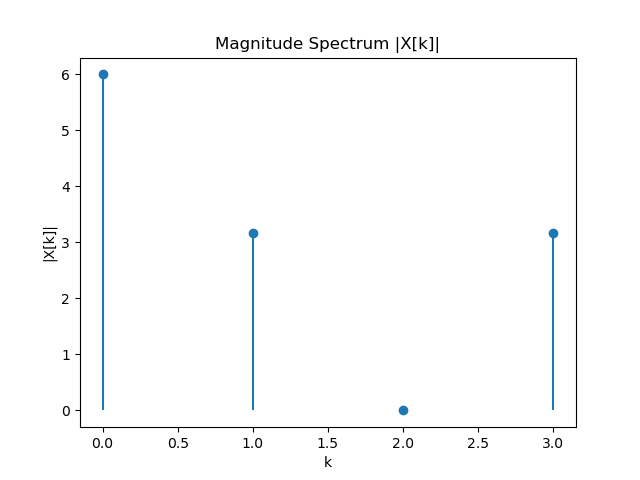
\includegraphics[width=\columnwidth, height=0.8\textheight, keepaspectratio]{figs/fig1.png}
   \label{fig:Beamer/figs/fig1.png}
\end{frame}

\end{document}
